%Please use LuaLaTeX or XeLaTeX
\documentclass[11pt,aspectratio=169]{beamer}

\title{Theta Functions, Kronecker Functions, and Bilinear Relations}
\date[2023]{Riemann Surfaces \\ in Mathematical Physics}
\author{Artyom Lisitsyn}
\institute{D-PHYS}

\usetheme{eth}

\colorlet{titlefgcolor}{ETHBlue}
\colorlet{accentcolor}{ETHRed}

\usepackage{cancel}

\newcommand{\ee}[0]{\mathbf{e}}

\begin{filecontents}{\jobname.bib}
    @book{Ber06,
        Author = {Marco Bertola},
        Title = {Riemann Surfaces and Theta Functions},
        Year = {2006}}

    @thesis{Cha22,
        Author = {Zhi Cong Chan},
        Title = {Towards a Higher-Genus Generalization of the
        Kronecker Function Using Schottky Covers},
        Year = {2022}
    }

    @misc{BL13,
      title={Multiple Elliptic Polylogarithms},
      author={Francis C. S. Brown and Andrey Levin},
      year={2013},
      archivePrefix={arXiv},
      primaryClass={math.NT},
    }

    @article{Broedel_2022,
	year = 2022,
	publisher = {International Press of Boston},
	author = {Johannes Broedel and Andre Kaderli},
	title = {Amplitude recursions with an extra marked point},
	journal = {Communications in Number Theory and Physics}
    }

    @article{Broedel_2015,
	year = 2015,
	publisher = {Springer Science and Business Media {LLC}},
	author = {Johannes Broedel and Carlos R. Mafra and Nils Matthes and Oliver Schlotterer},
	title = {Elliptic multiple zeta values and one-loop superstring amplitudes},
	journal = {Journal of High Energy Physics}
    }

    @article{Mat19,
    author = {Matthes, Nils},
    title = {An algebraic characterization of the Kronecker function},
    journal = {Research in the Mathematical Sciences},
    volume = {6},
    number = {3},
    pages = {24},
    year = {2019},
    ISSN = {2197-9847},
    }

    @book{ComputationalSchottky,
        title={Computational Approach to Riemann Surfaces},
        author={Alexander I. Bobenko and Christian Klein},
        year={2011},
        publisher={Lecture Notes in Mathematics. Springer Berlin Heidelberg}
    }
\end{filecontents}
\usepackage[backend=bibtex,style=authoryear, defernumbers=true]{biblatex}
\addbibresource{\jobname.bib}
\begin{document}

% Find better title image?
\def\titlefigure{assets/ThetaBigMonoCrop.png}
\titleframe{}

\tocframe{}

\section{Abel's map}

\begin{frame}{Holomorphic Differentials}
    \begin{block}{Definition and existence of holomorphic differentials}
        \vspace{-1em}
        \[\text{Definition: } \omega = f_\alpha dz_\alpha = f_\beta dz_\beta , \quad f \text{ holomorphic}\]
        \[\text{Existence: } \dim \mathcal H^1 = g \text{ (genus of compact Riemann surface)}\]
    \end{block}

    \begin{columns}[onlytextwidth]
        \begin{column}{0.55\textwidth}
            \emph{Proof outline:}
            \begin{itemize}
                \item $\dim \mathcal H^1 \leq \text{\# of a-cycles} = g$
                \item $\text{\# of harmonic differentials} = \dim H \geq 2g$
                \item $h = f dz + g d \bar z \implies \dim H = 2 \dim \mathcal H^1$
                \item $g \leq \dim \mathcal H^1 \leq g \implies \dim \mathcal H^1 = g$
            \end{itemize}
            \emph{Normalization \& period matrix:}
            \[ \int_{a_i} \omega_j = \delta_{ij} \]
            \[ \int_{b_i} \omega_j = \tau_{ij} \]
        \end{column}
        \begin{column}{0.45\textwidth}
            \center{}
            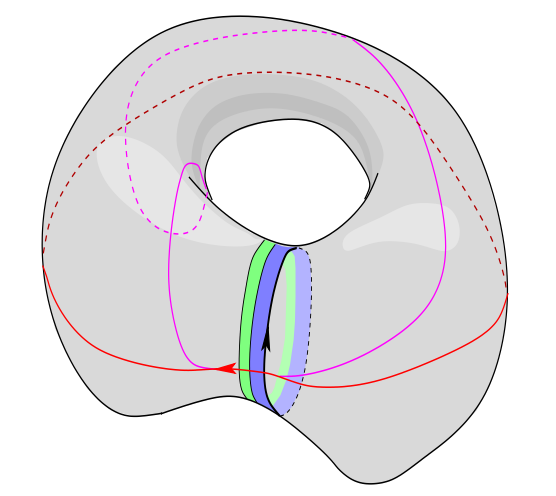
\includegraphics[width=0.8\columnwidth]{assets/HarmonicDifferential.png}
            
            \tiny Regions used to define harmonic differentials

            \cite{Ber06}
        \end{column}
    \end{columns}
\end{frame}

\begin{frame}{Abel's map}{\tiny \cite{Ber06} Section 4.2}
    \begin{columns}
        \begin{column}{0.55\textwidth}
            \begin{block}{Formal definition of Abel's map}
                For a particular choice of a point $P_0$ on the fundamental domain $\mathcal L$, using the normalized harmonic differentials $\omega_i$, we have Abel's map
                \[
                    \mathbf{u} : \mathcal L \rightarrow \mathbb{C}^g ,
                    \quad P \mapsto \begin{pmatrix} \int_{P_0}^P \omega_1 \\ \vdots \\ \int_{P_0}^P \omega_g \end{pmatrix}
                \]
            \end{block}
        \end{column}
        \begin{column}{0.45\textwidth}
            \center

            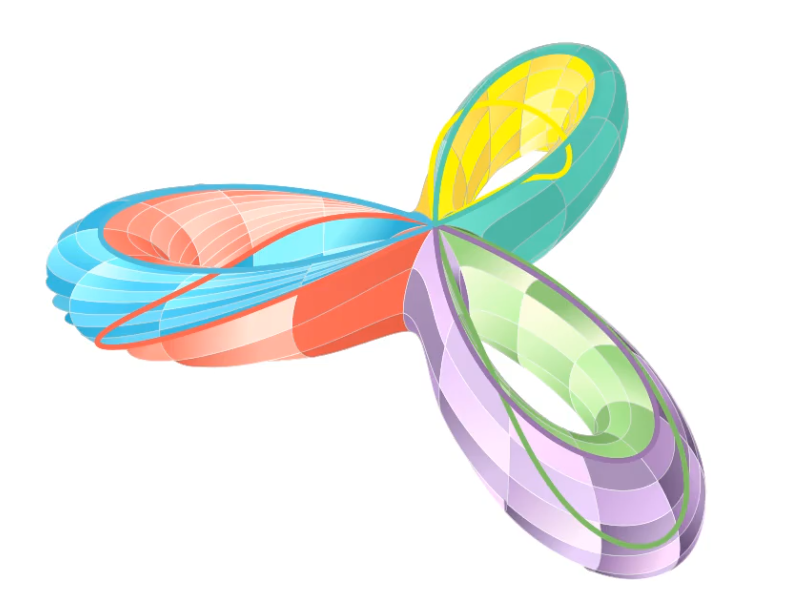
\includegraphics[width=0.7\columnwidth]{assets/Genus3Surface.png}

            \tiny Genus 3 surface
        \end{column}
    \end{columns}

    \emph{Analytic continuation beyond the fundamental domain:}
    \[\mathbf{u}(P+a_i) = \mathbf{u}(P) + \begin{pmatrix} \int_{a_i} \omega_1 \\ \vdots \end{pmatrix} = \mathbf{u}(P) + \begin{pmatrix} \delta_{i1} \\ \vdots \end{pmatrix}\]
    \[\mathbf{u}(P+b_i) = \mathbf{u}(P) + \begin{pmatrix} \tau_{i1} \\ \vdots \end{pmatrix}\]
\end{frame}

\begin{frame}[noframenumbering]{Abel's map}{\tiny \cite{Ber06} Section 4.2}
    \begin{columns}
        \begin{column}{0.55\textwidth}
            \begin{block}{Formal definition of Abel's map}
                For a particular choice of a point $P_0$ on the fundamental domain $\mathcal L$, using the normalized harmonic differentials $\omega_i$, we have Abel's map
                \[
                    \mathbf{u} : \mathcal L \rightarrow \mathbb{C}^g ,
                    \quad P \mapsto \begin{pmatrix} \int_{P_0}^P \omega_1 \\ \vdots \\ \int_{P_0}^P \omega_g \end{pmatrix}
                \]
            \end{block}
        \end{column}
        \begin{column}{0.45\textwidth}
            \center

            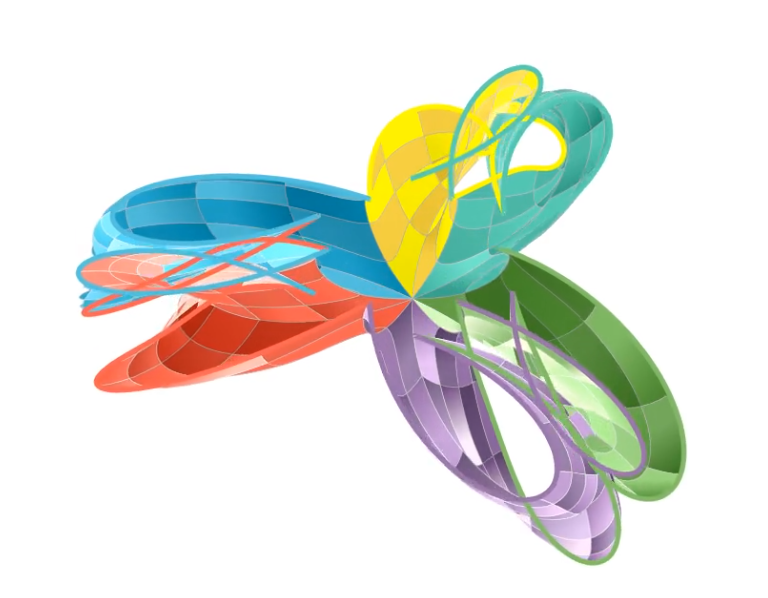
\includegraphics[width=0.7\columnwidth]{assets/Genus3Intermediate.png}

            \tiny Unfolding Genus 3 Surface
        \end{column}
    \end{columns}

    \emph{Analytic continuation beyond the fundamental domain:}
    \[\mathbf{u}(P+a_i) = \mathbf{u}(P) + \begin{pmatrix} \int_{a_i} \omega_1 \\ \vdots \end{pmatrix} = \mathbf{u}(P) + \begin{pmatrix} \delta_{i1} \\ \vdots \end{pmatrix}\]
    \[\mathbf{u}(P+b_i) = \mathbf{u}(P) + \begin{pmatrix} \tau_{i1} \\ \vdots \end{pmatrix}\]
\end{frame}

\begin{frame}[noframenumbering]{Abel's map}{\tiny \cite{Ber06} Section 4.2}
    \begin{columns}
        \begin{column}{0.55\textwidth}
            \begin{block}{Formal definition of Abel's map}
                For a particular choice of a point $P_0$ on the fundamental domain $\mathcal L$, using the normalized harmonic differentials $\omega_i$, we have Abel's map
                \[
                    \mathbf{u} : \mathcal L \rightarrow \mathbb{C}^g ,
                    \quad P \mapsto \begin{pmatrix} \int_{P_0}^P \omega_1 \\ \vdots \\ \int_{P_0}^P \omega_g \end{pmatrix}
                \]
            \end{block}
        \end{column}
        \begin{column}{0.45\textwidth}
            \center

            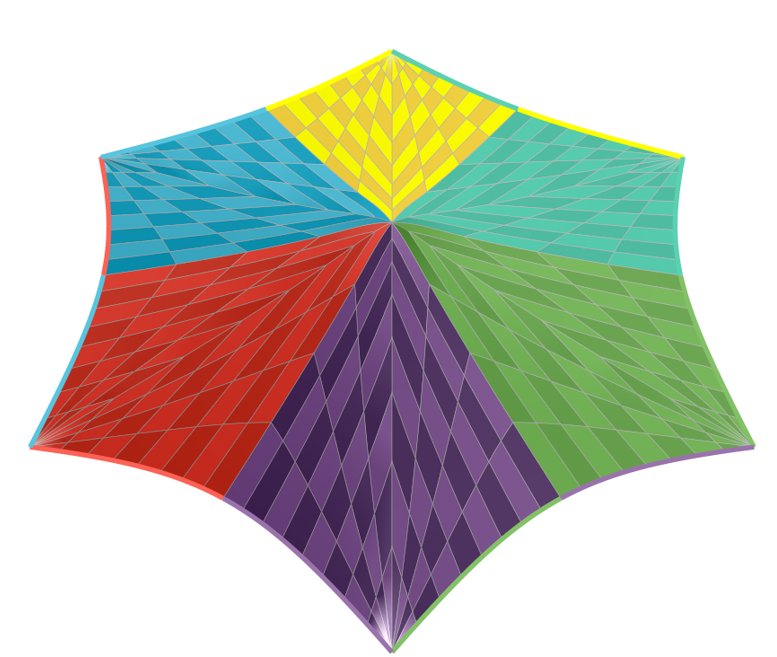
\includegraphics[width=0.7\columnwidth]{assets/Genus3Domain.png}

            \tiny Genus 3 fundamental domain
        \end{column}
    \end{columns}

    \emph{Analytic continuation beyond the fundamental domain:}
    \[\mathbf{u}(P+a_i) = \mathbf{u}(P) + \begin{pmatrix} \int_{a_i} \omega_1 \\ \vdots \end{pmatrix} = \mathbf{u}(P) + \begin{pmatrix} \delta_{i1} \\ \vdots \end{pmatrix}\]
    \[\mathbf{u}(P+b_i) = \mathbf{u}(P) + \begin{pmatrix} \tau_{i1} \\ \vdots \end{pmatrix}\]
\end{frame}

\begin{frame}{Abel's map at genus 1}
    \begin{columns}[onlytextwidth]
        \begin{column}{0.55\textwidth}
            Appropriate differential
            \[\omega = dz\]
            
            Abel's map
            \[\mathbf{u}(z) = \int_0^z \omega = z\]
        \end{column}
        \begin{column}{0.45\textwidth}
            \center{}
            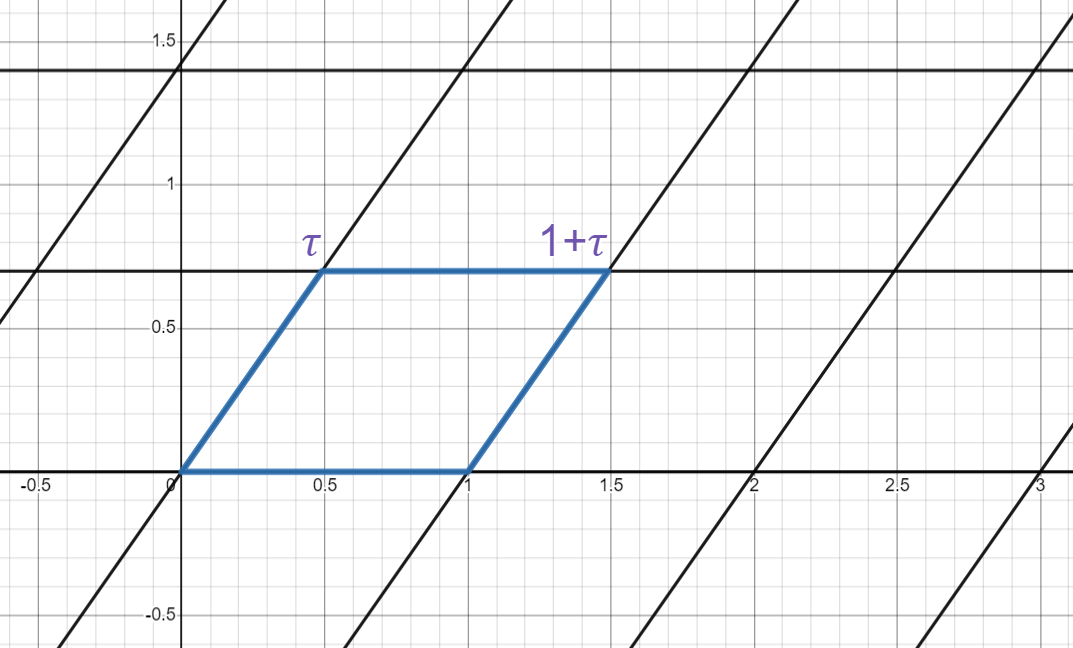
\includegraphics[width=\columnwidth]{assets/Domain.png}

            \tiny Fundamental domain and continuation at genus 1
        \end{column}
    \end{columns}

    {
    % \setbeamercolor{block body}
    \setbeamercolor{block title}{bg=ETHBlue}
    \setbeamercolor{block body}{bg=ETHBlue!25!white}
    \begin{block}{What about higher genus?}
        \begin{itemize}
            \item How do we represent the fundamental domain?
            \item What choice of differentials can we make?
            \item What consequences does this have for Abel's map?
        \end{itemize}
    \end{block}
    }
\end{frame}

\section{Theta functions}

\begin{frame}{Theta functions}{\tiny \cite{Ber06} Section 5.1}
    \begin{block}{Definition of the Theta function}
        Given a symmetric matrix $\tau$ with positive definite imaginary part, the Theta function is
        \[\Theta(\vec z, \tau) := \sum_{\vec n \in \mathbb Z^g} \ee \left( \frac{1}{2} \vec n^T \tau \vec n + \vec n^T \vec z \right) , \quad \ee(z) = \exp(2\pi i z)\]
    \end{block}
    % \pause
    \emph{Properties:} For $\vec \lambda \in \mathbb Z^g$

    \[\Theta(-\vec z) \overset{\vec n \mapsto -\vec n}{=} \Theta(\vec z)\]
    % \pause
    \[\Theta(\vec z + \vec \lambda) = \sum_{\vec n \in \mathbb Z^g} \cancelto{1}{\ee ( \vec n^T \vec \lambda)} \ee(\ldots) = \Theta(\vec z)\]
    % \pause
    \[\Theta(\vec z + \tau \vec \lambda) = \begin{bmatrix} \text{shift } \vec n \\ \text{use }\tau\text{ symmetry}\end{bmatrix} = \ee \left(- \frac{1}{2}\vec \lambda^T \tau \lambda-\vec \lambda^T \vec z\right)\Theta(\vec z)\]
\end{frame}

\begin{frame}{Theta function on a compact Riemann surface}{\tiny \cite{Ber06} Section 5.2}
    \begin{block}{Definition of Theta function on a compact Riemann surface}
        For a compact Riemann surface $\mathcal M$ of genus $g$, with period matrix $\tau$ and Abel's map $\mathbf{u}$, we can identify
        \begin{align*}
            \theta : \ & \mathcal M \rightarrow \mathbb C \\
            & P \mapsto \Theta(\mathbf{u}(P))
        \end{align*}
    \end{block}

    \emph{Properties:}
    \[ \theta(P + a_i) = \theta(P) \]

    \[ \theta(P + b_i) = \ee\left(- \frac{1}{2} \tau_{ii} - \mathbf{u}_i(P)\right)\theta(P) \]
\end{frame}

\begin{frame}{Theta function at genus 1}
    \begin{columns}[onlytextwidth]
        \begin{column}{0.55\textwidth}
            \[\theta(z) = \sum_{n \in \mathbb Z} \ee\left(\frac{1}{2}n^2 \tau + n z\right)\]

            \[\theta(z)=\theta(-z)\]
            \[\theta(z+1)=\theta(z)\]
            \[\theta(z+\tau)=\ee\left(-\frac{1}{2}\tau-\xi\right)\theta(z)\]
        \end{column}
        \begin{column}{0.45\textwidth}
            \center{}
            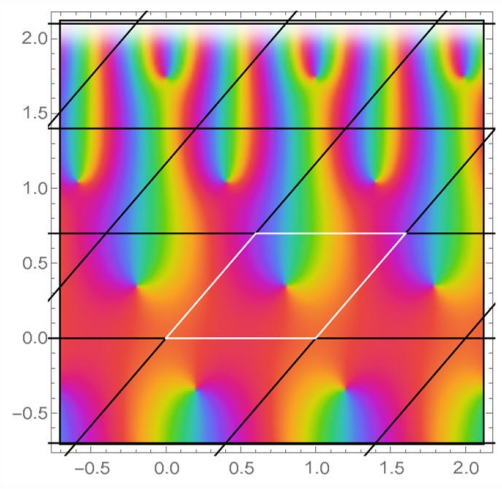
\includegraphics[width=0.7\columnwidth]{assets/genus1theta.png}

            \tiny Theta function for $\tau = 0.7+0.6i$
            
            \cite{Cha22}
        \end{column}
    \end{columns}

    {
    % \setbeamercolor{block body}
    \setbeamercolor{block title}{bg=ETHBlue}
    \setbeamercolor{block body}{bg=ETHBlue!25!white}
    \begin{block}{What about higher genus?}
        \begin{itemize}
            \item What does the Theta function look like at higher genus?
        \end{itemize}
    \end{block}
    }
\end{frame}

\begin{frame}{Theta function with characteristics}{\tiny \cite{Ber06} Section 5.1}
    \begin{block}{Definition of Theta function with characteristics}
        Consider vectors $ \epsilon ,  \epsilon' \in \mathbb R^g$.
        We can then define the Theta function with characteristics $ \epsilon$, $ \epsilon'$ as
        \[\Theta\begin{bmatrix} \epsilon \\  \epsilon'\end{bmatrix}(\vec z) := 
        \ee\left(\frac{1}{8}\epsilon^T \tau \epsilon + \frac{1}{2}\epsilon^T \vec z + \frac{1}{4}\epsilon^T  \epsilon'\right)
        \Theta\left(\vec z + \frac{\epsilon'}{2}+\frac{\tau\epsilon}{2}\right) = \begin{bmatrix}\vec n \mapsto \vec n+\epsilon \\ \vec z \mapsto \vec z + \epsilon' \end{bmatrix} \sum_{\vec n} \ee(...)\] 
    \end{block}
    % \pause
    \emph{Properties:}

    \[\Theta\begin{bmatrix}\epsilon \\ \epsilon'\end{bmatrix}(\vec z + \vec \alpha + \tau \vec \beta) =
    \ee\left(\frac{1}{2}(\epsilon^T \vec \alpha - \vec \beta^T \epsilon') - \frac{1}{2} \beta^T \tau \beta - \vec \beta \vec z\right)
    \Theta\begin{bmatrix}\epsilon \\ \epsilon'\end{bmatrix}(\vec z)\]
    % \pause
    \[\Theta\begin{bmatrix}\epsilon + 2\eta \\ \epsilon' + 2\eta' \end{bmatrix}(\vec z) = \exp(\pi i \epsilon^T \eta')
    \Theta\begin{bmatrix}\epsilon \\ \epsilon'\end{bmatrix}(\vec z) , \quad \eta,\eta' \in \mathbb Z^g\]
    % \pause
    \[\Theta\begin{bmatrix}\epsilon \\ \epsilon'\end{bmatrix}(-\vec z) = \exp(\pi i \epsilon^T \epsilon') \Theta\begin{bmatrix}\epsilon \\ \epsilon'\end{bmatrix}(\vec z) , \quad \epsilon,\epsilon' \in \mathbb Z^g\]
\end{frame}

\begin{frame}{Odd theta functions and zeros}
    \begin{columns}[onlytextwidth]
        \begin{column}{0.55\textwidth}
            \begin{align*}
                & \epsilon,\epsilon' \in \mathbb Z^g , \quad \epsilon^T \epsilon'\text{ is odd} \\
                & \Theta\begin{bmatrix}\epsilon \\ \epsilon'\end{bmatrix}(-\vec z) = \exp(\pi i \epsilon^T \epsilon') \Theta\begin{bmatrix}\epsilon \\ \epsilon'\end{bmatrix}(\vec z)
                \\
                & \implies \Theta\begin{bmatrix}\epsilon \\ \epsilon'\end{bmatrix}(\vec z) = -\Theta\begin{bmatrix}\epsilon \\ \epsilon'\end{bmatrix}(-\vec z)
                \\
                & \implies \Theta\begin{bmatrix}\epsilon \\ \epsilon'\end{bmatrix}(0) = \Theta\begin{bmatrix}\epsilon \\ \epsilon'\end{bmatrix}(\vec \alpha + \tau \vec \beta) = 0
                \\
                & \implies \Theta\left(\frac{\epsilon'}{2}+\frac{\tau\epsilon}{2}\right) = 0
            \end{align*}
        \end{column}
        \begin{column}{0.45\textwidth}
            \center{}
            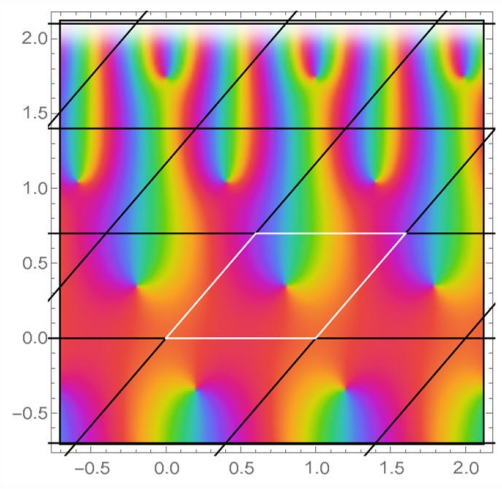
\includegraphics[width=0.7\columnwidth]{assets/genus1theta.png}

            \tiny Theta function for $\tau = 0.7+0.6i$
            
            \cite{Cha22}
        \end{column}
    \end{columns}

    {
        % \setbeamercolor{block body}
        \setbeamercolor{block title}{bg=ETHBlue}
        \setbeamercolor{block body}{bg=ETHBlue!25!white}
        \begin{block}{What about higher genus?}
            \begin{itemize}
                \item Which of the zeros located by odd characteristics are actually reached by Abel's map on compact Riemann surfaces of higher genus?
            \end{itemize}
        \end{block}
    }
\end{frame}

\begin{frame}{Odd theta function at genus 1}
    \begin{block}{Odd theta function at genus 1}
        We define
        \[\theta_1(z) = -\theta \begin{bmatrix} 1 \\ 1 \end{bmatrix}(z)\]
        It has equivalent definition
        \[\theta_1(z) = 2iq^{1/8} \sin(\pi z) \prod_j (1-q^j) (1-wq^j)(1-w^{-1}q^j) , \quad q=\ee(\tau),w=\ee{z}\]
    \end{block}
    \emph{Jacobi Triple Product:}
    % https://en.wikipedia.org/wiki/Jacobi_triple_product
    % https://en.wikipedia.org/wiki/Theta_function
    \[f(x,y) = \prod_{j>0} (1-x^{2m})(1+x^{2m-1}y^2)(1+x^{2m-1}y^{-2})\]
    \[f(x,xy) = \prod_{j>0} (1-x^{2m})(1+x^{2m+1}y^2)(1+x^{2m-3}y^{-2}) = \frac{1+x^{-1}y^{-2}}{1+xy^2} f(x,y) = x^{-1}y^{-2}f(x,y)\]
\end{frame}

\begin{frame}{Odd theta function at genus 1}
    \[f(x,y) = \prod_{j>0} (1-x^{2m})(1+x^{2m-1}y^2)(1+x^{2m-1}y^{-2})\]
    \[f(x,xy) = \prod_{j>0} (1-x^{2m})(1+x^{2m+1}y^2)(1+x^{2m-3}y^{-2}) = \frac{1+x^{-1}y^{-2}}{(1+xy^2)}f(x,y) = x^{-1}y^{-2}f(x,y)\]
    % \pause
    \[f(x,y) = \sum_{n=-\infty}^\infty c_n(x) y^{2n} \implies f(x,y) = xy^2 f(x,xy) = \sum_n c_n(x) x^{2n+1}y^{2n+2}\]
    \[\implies c_{n+1}(x) = x^{2n+1}c_n(x) \implies c_{n}(x) = c_0(x) x^{n^2} \implies f(x,y) = c_0(x) \sum_n x^{n^2} y^{2n}\]

    This relates the two forms of the theta function : $\prod_j (1-q^j) (1-wq^j)(1-w^{-1}q^j) \simeq \sum_n \ee(\tau)^{n^2} \ee(z)^{n}$

    {
        % \setbeamercolor{block body}
        \setbeamercolor{block title}{bg=ETHBlue}
        \setbeamercolor{block body}{bg=ETHBlue!25!white}
        \begin{block}{What about higher genus?}
            \begin{itemize}
                \item Are there similar Jacobi formulas for higher genus theta functions?
            \end{itemize}
        \end{block}
    }
\end{frame}

\begin{frame}{(Application) Decomposing meromorphic functions}{\tiny \cite{Cha22} Section 3.4 \& \cite{Ber06} Chapter 6}
    Rough outline of how to reproduce a function with divisor $(f) = \sum n_i P_i$
    \[ \begin{bmatrix}\text{Find function }t(z) \\ \text{with known simple zero}\end{bmatrix} \rightarrow \begin{bmatrix} g(z)=\prod t(P-P_i)^{n_i} \\ \text{respecting possible periodicity}\end{bmatrix} \rightarrow \left(\frac{f}{g}\right) = \emptyset \rightarrow \frac{f}{g} = \text{const.} \]
    Recall that $\deg((f)) = \sum n_i = 0$ for meromorphic functions, so extra factors can easily cancel.
    % \pause
    \vspace{+1em}
    \begin{columns}[t]
        \begin{column}{0.3\textwidth}
            Genus 0:
            \begin{itemize}
                \item $f(z) = C \prod (z-z_i)^{n_i}$
            \end{itemize}
        \end{column}

        \begin{column}{0.3\textwidth}
            Genus $>0$:
            \begin{itemize}
                \item $\Theta(\xi) = 0$
                \item $g_{P'} : P \mapsto \Theta(\mathbf{u}(P)-\mathbf{u}(P')+\xi)$
                \item $f(P) = C \prod \left(g_{P_i}(P)\right)^{n_i}$
            \end{itemize}
        \end{column}

        \begin{column}{0.35\textwidth}
            Genus 1:
            \begin{itemize}
                \item Decompose $z_i = \frac{b_i}{2} + \tau \frac{a_i}{2}$
                \item $f(z) = C \prod \left(\theta\begin{bmatrix}a_i \\ b_i\end{bmatrix}(z)\right)^{n_i}$
            \end{itemize}
        \end{column}
    \end{columns}
\end{frame}

\section{Kronecker function}

\begin{frame}{Analogous function for Genus 0}
    \[F(z,\alpha) = \frac{(z+\alpha)}{(z)(\alpha)}\]
    \[\downarrow\]
    \[\alpha F(z,\alpha) dz = \sum_{n=0,1} g^{(n)}(z) dz = dz + \frac{dz}{z}\]
    \[\downarrow\]
    \[\text{use differentials to calculate multiple polylogarithms}\]

    \begin{block}{Kronecker function at Genus 1}
        Elliptic version of what was shown above:
        \[\frac{\theta_1(z+\alpha)}{\theta_1(z)\theta_1(\alpha)}\]
    \end{block}
\end{frame}

\begin{frame}{Kronecker function}{\tiny \cite{BL13} Section 3.4}
    \begin{block}{Definitions of the Kronecker function}
        The Kronecker function $F(z,\alpha,\tau)$ has equivalent definitions
        \begin{enumerate}
            \item In terms of the odd theta function
            \[\frac{\theta_1'(0)\theta_1(z+\alpha)}{\theta_1(z)\theta_1(\alpha)}\]
            \item In terms of a sum over exponentials $F(\xi,\alpha,\tau)$
            \[-2\pi i \left(\frac{z}{1-z} + \frac{1}{1-w} + \sum_{m,n > 0} (z^m w^n - z^{-m} w^{-n}) q^{mn}\right) , \quad \begin{pmatrix} z \\ w \\ q \end{pmatrix} = \ee \begin{pmatrix}\xi \\ \alpha \\ \tau\end{pmatrix}\]
            \item In terms of a sum over Eisenstein functions and series
            \[\frac{1}{\alpha} \exp\left(-\sum_{j > 0} \frac{(-\alpha)^j}{j} (E_j(z,\tau) - e_j(\tau))\right)\]
        \end{enumerate}
    \end{block}
\end{frame}

\begin{frame}{Properties of the Kronecker function}{\tiny \cite{BL13} Section 3.4}
    {
        % \setbeamercolor{block body}
        \setbeamercolor{block title}{bg=ETHBlue}
        \setbeamercolor{block body}{bg=ETHBlue!25!white}
        \begin{block}{What about higher genus?}
            \begin{itemize}
                \item How can we define the Kronecker function at higher genus?
            \end{itemize}
        \end{block}
    }
    % \pause
    \emph{Periodicity Properties:}
    \[F(z+1,\alpha) = \frac{\theta_1'(0)\theta_1(z+\alpha+1)}{\theta_1(z+1)\theta_1(\alpha)} = F(z,\alpha)\]
    \[F(z+\tau,\alpha) = \frac{\theta_1'(0)\theta_1(z+\alpha+\tau)}{\theta_1(z+\tau)\theta_1(\alpha)} = \frac{\ee(-z-\alpha)}{\ee(-z)} F(z,\alpha)\]
    % \pause
    \begin{block}{The Fay Relation}
        \[F(z_1,\alpha_1)F(z_2,\alpha_2) = F(z_1,\alpha_1+\alpha_2)F(z_2-z_1,\alpha_2)+F(z_2,\alpha_1+\alpha_2)F(z_1-z_2,\alpha_1)\]
    \end{block}
\end{frame}

\begin{frame}{Setup for derivation of the Fay relation}{\tiny \cite{Mat19}}
    \[F(z_1,\alpha_1)F(z_2,\alpha_2) = F(z_1,\alpha_1+\alpha_2)F(z_2-z_1,\alpha_2)+F(z_2,\alpha_1+\alpha_2)F(z_1-z_2,\alpha_1)\]
    \vspace{-1em}
    \[\downarrow \text{rewrite using Theta functions} \downarrow\]
    \[\frac{\theta_1(z_1+\alpha_1)\theta_1(z_2+\alpha_2)}{\theta_1(z_1)\theta_1(\alpha_1)\theta_1(z_2)\theta_1(\alpha_2)}
    = \frac{\theta_1(z_1+\alpha_1+\alpha_2)\theta_1(z_2-z_1+\alpha_2)}{\theta_1(z_1)\theta_1(\alpha_1+\alpha_2)\theta_1(z_2-z_1)\theta_1(\alpha_2)}
    + \frac{\theta_1(z_1+\alpha_1+\alpha_2)\theta_1(z_1-z_2+\alpha_1)}{\theta_1(z_1)\theta_1(\alpha_1+\alpha_2)\theta_1(z_1-z_2)\theta_1(\alpha_1)}\]
    \[\downarrow \text{multiply common denominator and relabel} \downarrow \]
    \vspace{-2em}
    \begin{align*}
        & \theta_1(\alpha_0)\theta_1(\beta_0)\theta_1(\alpha_2+\beta_1)\theta_1(\alpha_2-\beta_1) + \\
        & \theta_1(\alpha_1)\theta_1(\beta_1)\theta_1(\alpha_0+\beta_2)\theta_1(\alpha_0-\beta_2) + \\
        & \theta_1(\alpha_2)\theta_1(\beta_2)\theta_1(\alpha_1+\beta_0)\theta_1(\alpha_1-\beta_0) = 0
    \end{align*}
    \vspace{-1em}
    \[\downarrow \text{long process involving odd and even theta functions at genus 1} \downarrow\]
    \[...\]
    {
        % \setbeamercolor{block body}
        \setbeamercolor{block title}{bg=ETHBlue}
        \setbeamercolor{block body}{bg=ETHBlue!25!white}
        \begin{block}{What about higher genus?}
            \begin{itemize}
                \item What does the Fay identity look like at higher genus when theta functions are more complicated?
            \end{itemize}
        \end{block}
    }
\end{frame}

\begin{frame}{Differentials from the Kronecker function}{\tiny \cite{Broedel_2015} Section 3.3.3}
    \[\alpha F(z,\alpha) dz = \sum_{n=0}^\infty g^{(n)}(z)dz \alpha^n \]
    \vspace{+1em}
    \[g^{(0)}(z) = 1\]
    \[g^{(1)}(z) = \pi \cot(\pi z) + 4\pi \sum_{m=1}^\infty \sin(2 \pi m z) \sum_{n=1}^\infty q^{mn}\]
    \[g^{(2)}(z) = -2\zeta_2 + 8 \pi^2 \sum_{m=1}^\infty \cos(2 \pi m z) \sum_{n=1}^\infty nq^{mn}\]
    \[\vdots\]
    % \pause
    \[\boxed{g^{(n)}(-z) = (-1)^n g^{(n)}(z)}\]
\end{frame}

\begin{frame}{Independence of the differentials}{\tiny \cite{BL13} Lemma 8}
    \[d(g^{(k+1)}(z)dz) = \nu \wedge (g^{(k)}(z)dz)\]

    Let us assume that the first $w$ differentials are not independent
    \[\sum_{k\leq w} c_{k} g^{(k)}(z) dz = 0\]

    Then, we find that
    \[ d\left(\sum_{k\leq w} c_{k} g^{(k)}(z) dz\right) = \nu \wedge \left(\sum_{k\leq (w-1)} c_{k} g^{(k)}(z) dz\right) = 0 \implies \sum_{k\leq (w-1)} c_{k} g^{(k)}(z) dz = 0 \]

    Thus,
    \[\sum_{k\leq (w-1)} c_{k} g^{(k)}(z) dz \neq 0 \implies \sum_{k\leq w} c_{k} g^{(k)}(z) dz \neq 0\]
    and since $c_0 g^{(0)}(z) dz \neq 0$, all the differentials are independent by induction.
\end{frame}

\begin{frame}{Fay relation for differentials (Kronecker to Decomposition)}
    \[F(z_1,\alpha_1)F(z_2,\alpha_2) = F(z_1,\alpha_1+\alpha_2)F(z_2-z_1,\alpha_2)+F(z_2,\alpha_1+\alpha_2)F(z_1-z_2,\alpha_1)\]
    \[\downarrow \text{decompose} \downarrow\]
    \begin{align*}
        \frac{1}{\alpha_1 \alpha_2}\left(\sum_{n=0}^\infty g^{(n)}(z_1) \alpha_1^n\right)\left(\sum_{n=0}^\infty g^{(n)}(z_2) \alpha_2^n\right)& = \\
        \frac{1}{(\alpha_1+\alpha_2)\alpha_2}\left(\sum_{n=0}^\infty g^{(n)}(z_1) (\alpha_1+\alpha_2)^n\right)\left(\sum_{n=0}^\infty g^{(n)}(z_2-z_1) \alpha_2^n\right)& + \\
        \frac{1}{(\alpha_1+\alpha_2)\alpha_1}\left(\sum_{n=0}^\infty g^{(n)}(z_2) (\alpha_1+\alpha_2)^n\right)\left(\sum_{n=0}^\infty g^{(n)}(z_1-z_2) \alpha_1^n\right)&
    \end{align*}
    
\end{frame}

\begin{frame}{Fay relation for differentials (decomposition to power matching)}
    \begin{align*}
        (\alpha_1+\alpha_2)\left(\sum_{n=0}^\infty g^{(n)}(z_1) \alpha_1^n\right)\left(\sum_{n=0}^\infty g^{(n)}(z_2) \alpha_2^n\right)& = \\
        \alpha_1\left(\sum_{n=0}^\infty g^{(n)}(z_1) (\alpha_1+\alpha_2)^n\right)\left(\sum_{n=0}^\infty g^{(n)}(z_2-z_1) \alpha_2^n\right)& + \\
        \alpha_2\left(\sum_{n=0}^\infty g^{(n)}(z_2) (\alpha_1+\alpha_2)^n\right)\left(\sum_{n=0}^\infty g^{(n)}(z_1-z_2) \alpha_1^n\right)&
    \end{align*}
    \[\downarrow \text{match coefficients of }\alpha_1^m \alpha_2^n \downarrow\]
    \begin{align*}
        g^{(m-1)}(z_1) g^{(n)}(z_2) + g^{(m)}(z_1) g^{(n-1)}(z_2) = \sum_{r=0}^n \begin{pmatrix} m-1+r \\ r \end{pmatrix} g^{(m-1+r)}(z_1) g^{(n-r)}(z_2-z_1)& + \\
        \sum_{r=0}^m \begin{pmatrix} n-1+r \\ r \end{pmatrix} g^{(n-1+r)}(z_2) g^{(m-r)}(z_1-z_2)&
    \end{align*}
\end{frame}

\begin{frame}{Fay relation for differentials (power matching to final form)}
    \begin{align*}
        g^{(m-1)}(z_1) g^{(n)}(z_2) + g^{(m)}(z_1) g^{(n-1)}(z_2) = \sum_{r=0}^n \begin{pmatrix} m-1+r \\ r \end{pmatrix} g^{(m-1+r)}(z_1) g^{(n-r)}(z_2-z_1)& + \\
        \sum_{r=0}^m \begin{pmatrix} n-1+r \\ r \end{pmatrix} g^{(n-1+r)}(z_2) g^{(m-r)}(z_1-z_2)&
    \end{align*}
    \[\downarrow ????? \downarrow\]
    \begin{align*}
        g^{(m)}(z_1) g^{(n)}(z_2) = (-1)^{n+1} g^{(m+n)}(z_1-z_2)& \\
         +\sum_{r=0}^m \begin{pmatrix} m+r-1 \\ r \end{pmatrix} g^{(m+r)}(z_1) g^{(n-r)}(z_2-z_1) & \\
         +\sum_{r=0}^m \begin{pmatrix} n+r-1 \\ r \end{pmatrix} g^{(n+r)}(z_2) g^{(m-r)}(z_1-z_2) & 
    \end{align*}
    \[z_1 = t-x \quad ; \quad z_2 = t \implies \text{repeated }t\text{ dependence} \rightarrow \text{repeated }x\text{ dependence}\]
\end{frame}

\begin{frame}{Periodicity instead of holomorphicity}{\tiny \cite{Broedel_2015} Section 3.2.3}
    \begin{block}{Elliptic version of Kronecker function}
        \[\Omega(z,\alpha) = \ee\left(\alpha \frac{\Im(z)}{\Im(\tau)}\right) F(z,\alpha)\]
        \vspace{+1em}
        \[\Omega(z+1,\alpha) = \ee\left(\alpha \frac{\Im(z+1)}{\Im(\tau)}\right) F(z+1,\alpha) = \Omega(z+1,\alpha)\]
        \[\Omega(z+\tau,\alpha) = \ee\left(\alpha \frac{\Im(z+\tau)}{\Im(\tau)}\right) F(z+1,\alpha) = \ee(\alpha) \ee\left(\alpha \frac{\Im(z)}{\Im(\tau)}\right) \ee(-\alpha) F(z,\alpha) = \Omega(z,\alpha)\]
    \end{block}
    % \pause
    Similarly, we find
    \[ \alpha \Omega(z,\alpha) = \sum_{n=0}^\infty f^{(n)}(z)dz \alpha^n \]
    for perfectly elliptic, but non-holomorphic $f$.

\end{frame}

\begin{frame}{Application of properties}
    \begin{columns}
        \begin{column}{0.5\textwidth}
            Properties of differentials:
            \begin{itemize}
                \item Periodic or quasi-periodic, with particular $\tau$ \\
                $\rightarrow$ faithful to compact Riemann surface
                \item Integrability and independence \\
                $\rightarrow$ suitable for homotopy-invariant integrals
                \item Constant ($g^{(0)}$) and simple pole ($g^{(1)}$) \\
                $\rightarrow$ constructing elliptic polylogarithms
                \item Fay relation \\
                $\rightarrow$ rearranging dependence for integral evaluation
            \end{itemize}
        \end{column}
        \begin{column}{0.45\textwidth}
            \center{}
            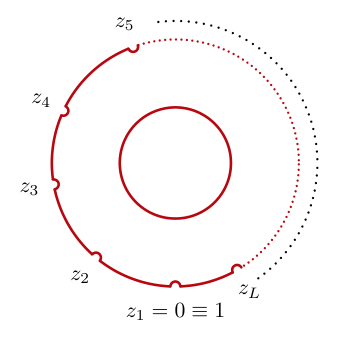
\includegraphics[width=0.7\columnwidth]{assets/Annulus.png}

            \tiny Annulus from open string

            \cite{Broedel_2022}
        \end{column}
    \end{columns}
\end{frame}

\section{Striving for higher genus}

\begin{frame}{Why we care about higher genus}
    \center{}
    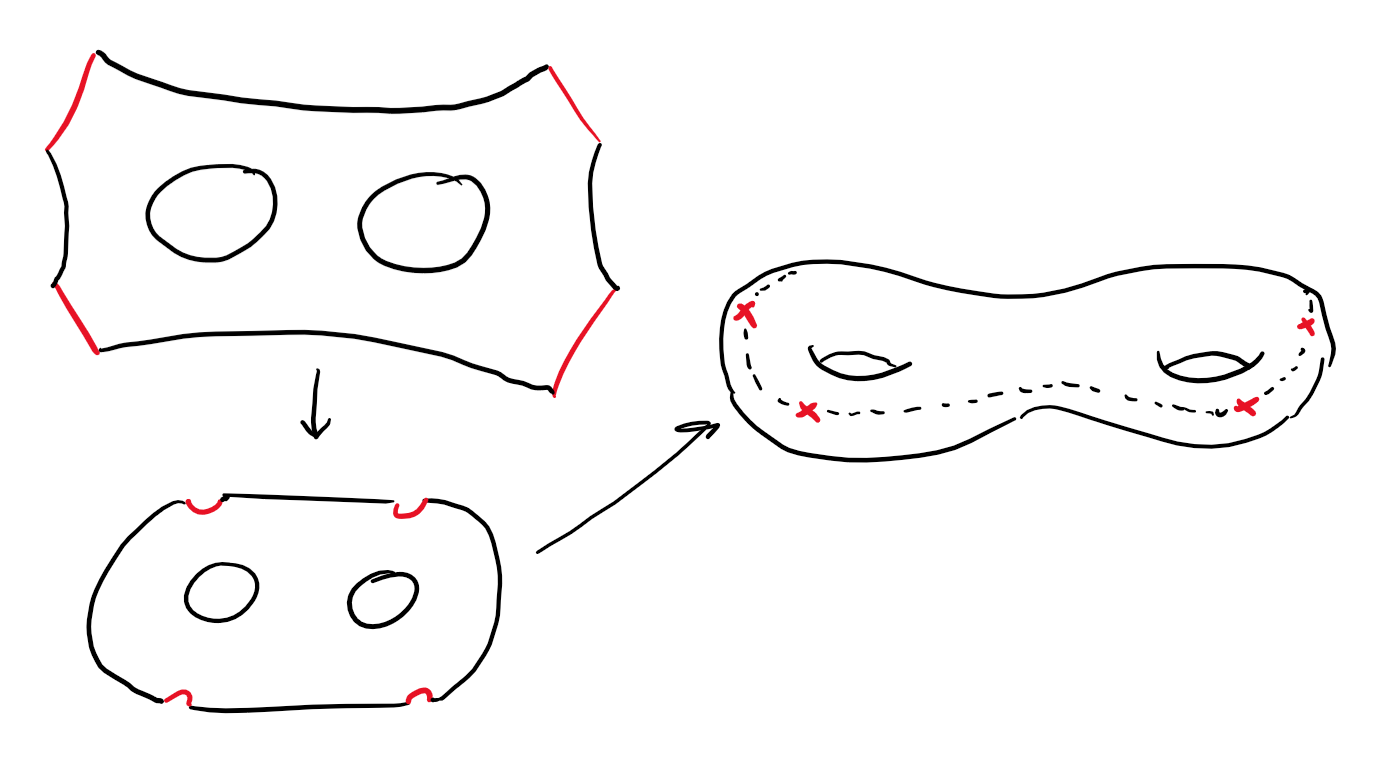
\includegraphics[width=0.7\columnwidth]{assets/MyGenus2.png}

    \tiny Sketch of analogous construction for genus 2
\end{frame}

\begin{frame}{Questions gathered so far}
    {
        % \setbeamercolor{block body}
        \setbeamercolor{block title}{bg=ETHBlue}
        \setbeamercolor{block body}{bg=ETHBlue!25!white}
        \begin{block}{What about higher genus?}
            \begin{itemize}
                \item How do we represent the fundamental domain?
                \item What choice of differentials can we make?
                \item What consequences does this have for Abel's map?
                \item What does the Theta function look like at higher genus?
                \item Which of the zeros located by odd characteristics are actually reached by Abel's map on compact Riemann surfaces of higher genus?
                \item Are there similar Jacobi formulas for higher genus theta functions?
                \item How can we define the Kronecker function at higher genus?
                \item What does the Fay identity look like at higher genus when theta functions are more complicated?
            \end{itemize}
        \end{block}
    }
\end{frame}

\begin{frame}{Questions gathered so far}
    {
        % \setbeamercolor{block body}
        \setbeamercolor{block title}{bg=ETHBlue}
        \setbeamercolor{block body}{bg=ETHBlue!25!white}
        \begin{block}{What about higher genus?}
            \begin{itemize}
                \item $\checkmark$ How do we represent the fundamental domain? 
                \item $\checkmark$ What choice of differentials can we make?
                \item $\checkmark$ What consequences does this have for Abel's map?
                \item What does the Theta function look like at higher genus?
                \item Which of the zeros located by odd characteristics are actually reached by Abel's map on compact Riemann surfaces of higher genus?
                \item Are there similar Jacobi formulas for higher genus theta functions?
                \item $\sim$ How can we define the Kronecker function at higher genus?
                \item What does the Fay identity look like at higher genus when theta functions are more complicated?
            \end{itemize}
        \end{block}
    }
\end{frame}

\begin{frame}{Schottky group}{\tiny \cite{ComputationalSchottky} and \cite{Cha22}}
    \begin{block}{Schottky group}
        Choosing mutually disjoint discs $\{D_i,D_i'\}$ with interiors $\{\mathring{D}_i,\mathring{D}_i'\}$ on a Riemann sphere,
        we can choose mobius transformations $\gamma_i$ such that the exterior of $D_i$ is mapped to the interior of $D_i'$
        \[\gamma_i \in \text{PSL}_2(\mathbb C) , \quad \gamma_i : z \mapsto \frac{az+b}{cz+d}\]
        \[\gamma_i(\bar C \setminus \mathring{D}_i) = D_i'\]
        \[\gamma_i(\partial D_i) = \partial D_i'\]

        The transformations formed by composition of $\gamma_i$ form a group called a \textbf{Schottky group}, usually denoted as $\Gamma$.
    \end{block}

    \center{}
    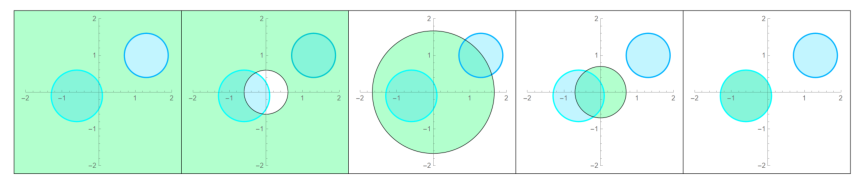
\includegraphics[width=0.7\columnwidth]{assets/ChanSchottkyGroup.png}

    \tiny Mobius transformations mapping outside of one disc to inside of another

    \cite{Cha22}
\end{frame}

\begin{frame}{Schottky cover}{\tiny \cite{ComputationalSchottky} and \cite{Cha22}}
    \begin{block}{Schottky cover}
        Given a Schottky group $\Gamma$ with associated discs $\{D_i,D_i'\}_{i=1}^g$ we can define
        \[F := \bar {\mathbb C} \setminus \bigcup_i (\overset{\circ}{D}_i \cup \overset{\circ}{D}_i') \quad ; \quad \Omega := \bigcup_{\gamma \in \Gamma} \gamma(F)\]
        Then, $\mathcal M := \Omega / \Gamma$ is a Riemann surface of genus $g$ with fundamental domain $F$.
    \end{block}
    \center{}
    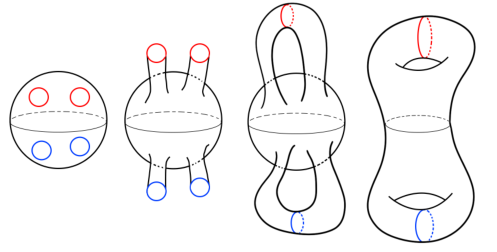
\includegraphics[width=0.6\textwidth]{assets/ChanSchottkyCover.png}

    \tiny Schotty cover mapping to compact Riemann surface

    \cite{Cha22}
\end{frame}

\begin{frame}{Schottky cover}{\tiny \cite{Cha22}}
    \center{}
    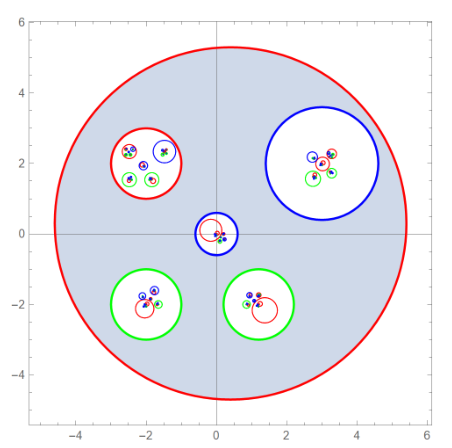
\includegraphics[width=0.5\textwidth]{assets/ChanSchottkyCover2.png}

    \tiny Schotty cover visual for verbal explanation

    \cite{Cha22}
\end{frame}

\begin{frame}{Differentials and Abel's map}{\tiny \cite{ComputationalSchottky} and \cite{Cha22}}
    We can define cosets of $\Gamma$
    \[\Gamma / \Gamma_i = \{\gamma_{j_1}^{n_1}\cdots \gamma_{j_k}^{n_k}: \gamma_{j_k} \neq \gamma_i\}\]
    \[\Gamma_i \setminus \Gamma  = \{\gamma_{j_1}^{n_1}\cdots \gamma_{j_k}^{n_k}: \gamma_{j_1} \neq \gamma_i\}\]
    % \pause
    And use these to define holomorphic differentials using fixed points $P_i$
    \[\omega_i = \frac{1}{2\pi i}\sum_{\gamma \in \Gamma / \Gamma_i} \left(\frac{1}{z-\gamma(P_i')} - \frac{1}{z-\gamma(P_i)}\right)dz = \frac{1}{2\pi i}\sum_{\gamma \in \Gamma_i \setminus \Gamma } \left(\frac{1}{\gamma(z)-P_i'} - \frac{1}{\gamma(z)-P_i}\right)d(\gamma(z))\]
    % \pause
    Which can then be used to define Abel's map
    \[u_i[p] = \int_{p_0}^p \omega_i = \frac{1}{2\pi i} \sum_{\gamma \in \Gamma/\Gamma_i} \ln \{p,\gamma(P_i'),p_0,\gamma(P)\}\]
    where
    \[\{a,b,c,d\} = \frac{(a-b)(c-d)}{(a-d)(c-b)}\]
\end{frame}

\begin{frame}{Attempt at a Kronecker function}{\tiny \cite{Cha22}}
    Focusing on three of the conditions:
    \begin{enumerate}
        \item Generalized Kronecker function should be quasi-periodic
        \item Generalized Kronecker function should reduce to aforementioned genus 1 form
        \item Generalized Kronecker function should satisfy integrability in a particular way
    \end{enumerate}
    \[K(z,\{w_1,...,w_g\}|\Gamma) = \sum_{\gamma \in \Gamma} \frac{\gamma'(z)}{\gamma(z)-1} w_1^{\mathrm{ord}_1\gamma}...w_g^{\mathrm{ord}_g\gamma}\]
    
    At Genus 1, for $\gamma : z \mapsto \ee(\tau) z = qz$
    \[K(z,w|\Gamma) = \sum_{n \in \mathbb Z} \frac{q^n}{q^n z - 1} w^n = \cdots = \frac{1}{z} \left[1 - \frac{1}{1-z} - \frac{1}{1-w} - \sum_{m,n > 0} q^{mn} (z^m w^n - z^{-m} w^{-n})\right]\]
    Recall
    \[F(\xi,\alpha) = -2\pi i \left(\frac{z}{1-z} + \frac{1}{1-w} + \sum_{m,n > 0} (z^m w^n - z^{-m} w^{-n}) q^{mn}\right) \quad , \quad \begin{pmatrix} z \\ w \\ q \end{pmatrix} = \ee \begin{pmatrix}z \\ \alpha \\ \tau\end{pmatrix}\]
\end{frame}

\begin{frame}{Open questions}
    \textbf{Obtaining the Kronecker function in terms of theta functions}
    \begin{itemize}
        \item Choice of characters, description of theta's behavior
        \item Existing attempts inspiring representation with theta functions
    \end{itemize}

    \textbf{More detail in Schottky cover description}
    \begin{itemize}
        \item Matching Schottky fundamental domain with usual fundamental polygon
        \item Alternative choices for generalized Kronecker function
    \end{itemize}

    \textbf{Connection to algebraic curves}
    \begin{itemize}
        \item Mapping to other language of describing Riemann surfaces
    \end{itemize}
\end{frame}

\begin{frame}{References}
    \printbibliography{}
\end{frame}

\end{document}